% !TeX root = surprises.tex

\selectlanguage{hebrew}


\chapter[\R{האם משולשים עם אותו שטח ואותו היקף חופפים?}]{האם משולשים עם אותו שטח\\
ואותו היקף חופפים?}
\label{c.congruent}
%%%%%%%%%%%%%%%%%%%%%%%%%%%%%%%%%%%%%%%%%%%%%%%%%%%%%%%%%%%%%%%


האם משולשים עם אותו שטח ואותו היקף חופפים? לא בהכרח: לשני המשולשים הלא-חופפים עם הצלעות
$(17,25,28)$
ו-%
$(20,21,27)$
היקף
$70$
ושטח 
$210$
(איור%
~\ref{f.congruent-first-example}).
פרק זה מראה שנתון משולש עם אורכי צלעות רציונליים, ניתן לבנות משולש לא-חופף עם אורכי צלעות רציונליים, ועם אותו היקף ושטח. את השיטה נדגים על דוגמה ונראה שלמשולש עם הצלעות 
$(3,4,5)$
ולמשולש עם הצלעות
$(\frac{156}{35},\frac{101}{21},\frac{41}{15})$
אותו היקף
$12$
ואותו שטח
$6$.

\begin{figure}[tb]
\begin{center}
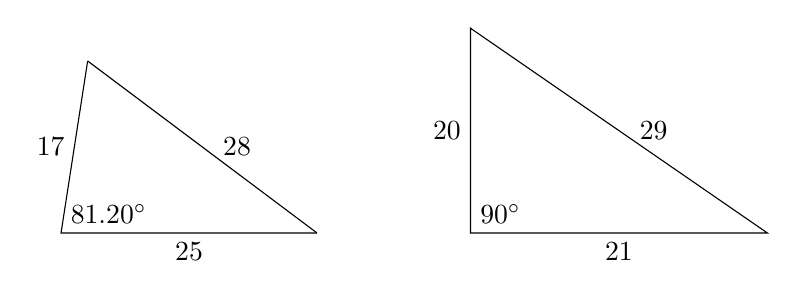
\begin{tikzpicture}[scale=1.3]
\coordinate (A1) at (0,0);
\node[above right] at (A1) {$81.20^\circ$};
\coordinate (B1) at (2.5cm,0);
\coordinate (C1) at (81.20:1.7cm);
\draw (B1) -- node[below] {$25$} (A1) -- node[left] {$17$} (C1);
\draw (B1) -- node[right,xshift=4pt] {$28$} +(143.13:2.8cm);
\begin{scope}[xshift=4cm]
\coordinate (A2) at (0,0);
\node[above right] at (A2) {$90^\circ$};
\coordinate (B2) at (2.9cm,0);
\coordinate (C2) at (0,2cm);
\draw (B2) -- node[below] {$21$} (A2) -- node[left] {$20$} (C2) -- node[right,xshift=4pt] {$29$} cycle;
\end{scope}
\end{tikzpicture}
\end{center}
\caption{משולשים לא חופפים עם אותו שטח ואותו הקיף}\label{f.congruent-first-example}
\end{figure}

\section{ממשולש לעקומה אליפטית}

חוצי הזווית של משולש נחתכים בנקודה 
$O$
הנקראת מרכז המעגל המוקף של המשולש
\L{(incenter)} (איור%
~\ref{f.inscribed}).%
\footnote{%
כך לפי המילון של האקדמיה ללשון העברית. מקובל לקרוא לנקודה: המרכז של המעגל החסום על ידי המשולש.%
}
נוריד גבהים מ-%
$O$
לצלעות. לגבהים אורך
$r$,
הרדיוס של המעגל החסום. הגבהים וחוצי הזווית מייצרים שלושה זוגות של משולשים ישרים חופפים:
\[
\triangle AOB'\cong \triangle AOC',\quad \triangle BOA'\cong \triangle BOC', \quad \triangle COA'\cong \triangle COB'\,.
\]
\begin{figure}[tb]
\begin{center}
\begin{tikzpicture}[baseline=-6mm,scale=2.25]
% Draw base and path two lines at known angles
\draw (0,0) coordinate (a) node[xshift=-6pt] {$A$} -- (0:6) coordinate (b) node[xshift=6pt] {$B$};
\path[name path=ac] (a) -- +(50:4);
\path[name path=bc] (b) -- +(150:5);
% Get their intersection and draw lines between vertices
\path[name intersections={of=ac and bc,by=c}];
\node[above] at (c) {$C$};
\draw (a) -- (c) -- (b) -- (a);
% Label angles with tick marks
\draw (a) ++(0:4mm) arc (0:50:4mm);
\draw (a) ++(10:3.5mm) -- +(10:1mm);
\draw (a) ++(15:3.5mm) -- +(15:1mm);
\draw (a) ++(35:3.5mm) -- +(35:1mm);
\draw (a) ++(40:3.5mm) -- +(45:1mm);
\draw (b) ++(150:5mm) arc (150:180:5mm);
\draw (b) ++(157.5:4.5mm) -- +(157.5:1mm);
\draw (b) ++(172.5:4.5mm) -- +(172.5:1mm);
\draw (c) ++(230:3mm) arc (230:330:3mm);
\draw (c) ++(250:2.5mm) -- +(250:1mm);
\draw (c) ++(255:2.5mm) -- +(255:1mm);
\draw (c) ++(260:2.5mm) -- +(260:1mm);
\draw (c) ++(300:2.5mm) -- +(300:1mm);
\draw (c) ++(305:2.5mm) -- +(305:1mm);
\draw (c) ++(310:2.5mm) -- +(310:1mm);
% Path bisectors of two lines
\path[name path=bia] (a) -- +(25:3.5);
\path[name path=bib] (b) -- +(165:5);
% Intersection of angle bisectors
\path [name intersections={of=bia and bib,by=center}];
% Draw angle bisectors to center
\draw (a) -- (center);
\draw (c) -- (center);
\draw (b) -- (center);
% Draw radii
\draw (center) -- node[left] {$r$} ($(a)!(center)!(b)$) node[below,yshift=-2pt] {$C'$} coordinate (ap);
\draw (center) -- node[left,yshift=-4pt] {$r$} ($(a)!(center)!(c)$) node[above left] {$B'$} coordinate (bp);
\draw (center) -- node[right] {$r$} ($(b)!(center)!(c)$) node[above right] {$A'$} coordinate (cp);
% Draw dots
\fill (center) circle (.5pt) node[above,xshift=3pt,yshift=6pt] {$O$};
\fill (a) circle (.5pt);
\fill (b) circle (.5pt);
\fill (c) circle (.5pt);
\fill (ap) circle (.5pt);
\fill (bp) circle (.5pt);
\fill (cp) circle (.5pt);
% Draw right angle squares
\draw (ap) -- ++(90:4pt) -- ++(0:4pt) -- ++(-90:4pt);
\draw (bp) -- ++(-40:4pt) -- ++(-130:4pt) -- ++(-220:4pt);
\draw (cp) -- ++(-30:4pt) -- ++(-120:4pt) -- ++(-210:4pt);
% Labels of angles
\node[above,xshift=5pt,yshift=21pt] at (center) {$\gamma/2$};
\node[above left,xshift=-4pt,yshift=21pt] at (center) {$\gamma/2$};
\node[above right,xshift=4pt,yshift=-5pt] at (center) {$\beta/2$};
\node[below right,yshift=-6pt] at (center) {$\beta/2$};
\node[left,xshift=-8pt,yshift=3pt] at (center) {$\alpha/2$};
\node[below left,xshift=2pt,yshift=-6pt] at (center) {$\alpha/2$};
% Labels of line segments (names of points are weird...)
\path (a) -- node[below,yshift=-2pt] {$u$} (ap);
\path (a) -- node[left, xshift=-2pt] {$u$} (bp);
\path (b) -- node[above,yshift=2pt]  {$v$} (cp);
\path (b) -- node[below,xshift=-2pt] {$v$} (ap);
\path (c) -- node[above,xshift=-2pt] {$w$} (bp);
\path (c) -- node[above,xshift=2pt]  {$w$} (cp);
% Labels of sides
\draw[<->] ($(a)+(0,-15pt)$) -- node[fill=white] {$c$} 
           ($(b)+(0,-15pt)$);
\draw[<->] ($(a)+(-12pt,10pt)$) -- node[fill=white] {$b$}
           ($(c)+(-12pt,10pt)$);
\draw[<->] ($(b)+(6pt,13pt)$) -- node[fill=white] {$c$}
           ($(c)+(6pt,13pt)$);
% Inscribed circle
\node[thick,dotted,draw,circle through=(ap)] at (center) {};
\end{tikzpicture}
\end{center}
\selectlanguage{hebrew}
\caption{מעגל חסום המוגדר על ידי חיתוך חוצי הזווית משולש}\label{f.inscribed}
\end{figure}
הגבהים מחלקים את הצלעות לקטעי קו.
$u,v,w$.
שלהן עם המעגל. השטח של
$\triangle ABC$
הוא סכום השטחים של 
$\triangle AOC, \triangle BOC, \triangle AOB$:
\begin{eqnlabels}
A &=& \frac{1}{2}(w+v)r + \frac{1}{2}(v+u)r + \frac{1}{2}(u+w)r\label{eq.area1}\\
&=& \frac{1}{2}\cdot 2(u+v+w)r\label{eq.area1a}\\
&=& \frac{1}{2} (a+b+c)r\label{eq.area1b}\\
&=& rs\,, \label{eq.area2}
\end{eqnlabels}
כאשר 
$s$
הוא מחצית היקף המשלוש
$\triangle ABC$. 
ניתן לבטא את 
$u,v,w$
באמצעות רדיוס המעגל והזוויות המרכזיות
$\alpha/2,\beta/2,\gamma/2$:
\begin{equation}\label{eq.uvw}
\tan \frac{\alpha}{2}= \frac{u}{r},\quad
\tan \frac{\beta}{2}= \frac{v}{r},\quad
\tan \frac{\gamma}{2} = \frac{w}{r}\,.
\end{equation}
כעת ניתן לבטא את מחצית ההיקף באמצעות הטנגנסים:
\[
s = u+v+w = r\tan \frac{\alpha}{2}+r\tan \frac{\beta}{2}+r\tan \frac{\gamma}{2} = r\left(\tan \frac{\alpha}{2}+\tan \frac{\beta}{2}+\tan \frac{\gamma}{2}\right)\,,
\]
ולפי משוואה~%
\ref{eq.area2}
השטח הוא:
\begin{equation}
A =sr=r^2\left(\tan \frac{\alpha}{2}+\tan \frac{\beta}{2}+\tan \frac{\gamma}{2}\right)\,.
\end{equation}
מ-%
$r=A/s$,
ניתן לכתוב את משוואה%
~\ref{eq.area2}
כ:
\begin{equation}
\tan \frac{\alpha}{2}+\tan \frac{\beta}{2}+\tan \frac{\gamma}{2} = \frac{A}{r^2} = \frac{A}{(A/s)^2} = \frac{s^2}{A}\,.\label{eq.area3}
\end{equation}
סכום הזוויות
$\alpha,\beta,\gamma$
הוא
$360^\circ$:
\begin{eqnlabels}
\gamma/2 &=& 360^\circ - (\alpha/2 + \beta/2)\\
\tan\gamma/2 &=& \tan(360^\circ - (\alpha/2 + \beta/2))\\
\tan\gamma/2&=& -\tan (\alpha/2 + \beta/2)\\
\tan\gamma/2&=& \frac{\tan\alpha/2 + \tan\beta/2}{\tan\alpha/2 \, \tan\beta/2-1}\,.\label{eq.tangent1}
\end{eqnlabels}
השתמשנו בנוסחה לטנגנס של החיבור של שתי זוויות (משפט%
~\ref{thm.tangent-sum}).

נפשט את הסימון על ידי הגדרת נעלמים עבור הטנגנסים:
\begin{equation}
\label{eq.variables-for-tangents}
x=\tan \frac{\alpha}{2},\quad
y=\tan \frac{\beta}{2},\quad
z=\tan \frac{\gamma}{2}\,.
\end{equation}
לפי משוואה~%
\ref{eq.tangent1}
ניתן לבטא את
$z=\tan \gamma/2$
כתלות ב-%
$x,y$:
\begin{equation}
z = \frac{x+y}{xy-1}\,.\label{eq.xy1}
\end{equation}
עם סימן זה משוואה~%
\ref{eq.area3}
היא:
\begin{equation}
x+y+\frac{x+y}{xy-1}=\frac{s^2}{A}\,.\label{eq.xy2}
\end{equation}
נתון ערכים קבועים של
$A$
ו-%
$s$,
האם קיימים פתרונות שונים למשוואה%
~\ref{eq.xy2}?

עבור משולש ישר-הזווית
$(3,4,5)$:
\[
\frac{s^2}{A} = \frac{\left(\frac{1}{2}(3+4+5)\right)^2}{\frac{1}{2}\cdot 3\cdot 4} = \frac{6^2}{6}=6\,.
\]
אם קיים פתרון אחר למשוואה%
~\ref{eq.xy2}
עם
$s^2/A=6$,
ניתן לכתוב אותו כ:
\begin{eqnlabels}
x+y+\frac{x+y}{xy-1}&=&6\\
x^2y + xy^2 -6xy + 6 &=& 0\,.\label{eq.elliptic}
\end{eqnlabels}
משוואה זו נקראת עקומה אליפטית
\L{(elliptic curve)}.

\section{פתרון המשוואה של העקומה האליפטית}

העקומה באיור~%
\ref{f.two-secants}
היא גרף חלקי של משוואה
\ref{eq.elliptic}.
כל נקודה על העקומה ברביע הראשון היא פתרון, כי אורכי הצלעות חייבים להיות חיוביים. הנקודות
$A,B,D$
מתאימות למשולש
$(3,4,5)$
כפי שנראה בסעיף%
~\ref{s.triangle-from-elliptic}.
כדי למצוא פתרונות רציונליים נוספים, נשתמש ב-%
\textbf{שיטת שני סקנסים}
\L{(\textbf{method of two secants})}.

\begin{figure}[tb]
\begin{center}
\begin{tikzpicture}[scale=1]
\draw[very thin,step=10mm] (-4,-4) grid (4,4);
\draw[thick] (-4,0) -- (4,0);
\draw[thick] (0,-4) -- (0,4);
\foreach \x in {-3,...,4}
  \node at (\x-.2,-.2) {\sm{\x}};
\foreach \y in {-3,...,-1}
  \node at (+.2,\y-.3) {\sm{\y}};
\foreach \y in {1,...,4}
  \node at (+.2,\y-.3) {\sm{\y}};

\draw[very thick,domain=.936:3.306,samples=200] plot (\x,{
(
  (6*\x-\x*\x)+
  sqrt(
   (\x*\x-6*\x)^2 -
   4*\x*6
  )
)/
(2*\x)
});

\draw[very thick,domain=.936:3.306,samples=100] plot (\x,{
(
  (6*\x-\x*\x)-
  sqrt(
   (\x*\x-6*\x)^2 -
   4*\x*6
  )
)/
(2*\x)
});

\draw[very thick,domain=-2.5:-.25,samples=100] plot (\x,{
(
  (6*\x-\x*\x)+
  sqrt(
   (\x*\x-6*\x)^2 -
   4*\x*6
  )
)/
(2*\x)
});

\coordinate (A) at (2,3);
\coordinate (B) at (1,2);
\coordinate (C) at (-1.5,-0.5);
\coordinate (D) at (3,2);
\coordinate (E) at (1.5,1.2);

\draw[very thick,dashed,red]  ($(C)!-.4!(A)$) -- ($(C)!1.2!(A)$);
\draw[very thick,dashed,blue] ($(C)!-.4!(D)$) -- ($(C)!1.2!(D)$);

\node[right,xshift=9pt,yshift=-5pt]  at (A)  {$A=(2,3)$};
\node[above left,xshift=-4pt]        at (B)  {$B=(1,2)$};
\node[right,xshift=23pt,yshift=-4]   at (C)  {$C=(-1.5,-0.5)$};
\node[right,xshift=8pt,yshift=-6pt]  at (D)  {$D=(3,2)$};
\node[below,xshift=15pt,yshift=-12pt] at (E) {$E=(1.5,1.2)$};
\vertexcolor{A}{red};
\vertexcolor{B}{red};
\vertexcolor{C}{purple};
\vertexcolor{D}{blue};
\vertexcolor{E}{blue!50!red};
\end{tikzpicture}
\end{center}
\selectlanguage{hebrew}
\caption{שיטת שני הסקנטים}\label{f.two-secants}
\end{figure}
נצייר סקנס דרך הנקודות
$A=(2,3)$
ו-%
$B=(1,2)$
שחותך את העקומה ב-%
$C=(-1.5,-0.5)$.
נקודה זו אינה פתרון כי הקואורדינטות שליליים. אם נצייר סקנס שני מ-%
$C$
ל-%
$D=(3,2)$,
החיתוך שלו עם העקומה ב-%
$E\approx(1.5,1.2)$
כן מהווה פתרון נוסף ונחשב בהמשך את הקואורדינטות.

המשוואה של הקו (האדום) דרך 
$A,B$
היא
$y=x+1$. 
נציב עבור 
$y$
במשוואה%
~\ref{eq.elliptic}:
\begin{eqn}
x^2(x+1) + x(x+1)^2 -6x(x+1) +6 &=&0\\
2x^3 -3x^2 -5x +6 &=&0\,.
\end{eqn}
מהנקודות
$A,B$
אנו יודעים שני שורשים
$x=2,x=1$,
ולכן ניתן לפרק את הפולינום ממעלה שלוש כך:
\[
(x-2)(x-1)(ax+b)=0\,,
\]
כאשר רק השורש השלישי לא ידוע.

נכפיל את הגורמים ונסיק ש-%
$a=2, b=3$
כי
$2x^3 -3x^2 -5x +6 = ax^3+\cdots+2b$.
הגורם השלישי הוא
$2x+3$
שנותן אל השורש השלישי
$x=-\frac{3}{2}$
ו-%
$y=x+1=-\frac{1}{2}$.
זאת הנקודה
$C=(-\frac{3}{2},-\frac{1}{2})$
בגרף.

המשוואה של הקו (הכחול) דרך
$D,C$
היא:
\begin{equation}
y = \frac{5}{9}x + \frac{1}{3}\,.\label{eq.second-secant}
\end{equation}
נציב עבור 
$y$
במשוואה 
~\ref{eq.elliptic}:
\begin{eqn}
x^2\left(\frac{5}{9}x + \frac{1}{3}\right) + x\left(\frac{5}{9}x + \frac{1}{3}\right)^2 -6x\left(\frac{5}{9}x + \frac{1}{3}\right) +6 &=&0\\
\frac{70}{81}x^3 - \frac{71}{27}x^2 - \frac{17}{9}x +6 &=&0\,.
\end{eqn}
מ-%
$C,D$
אנו יודעים שני שורשים
$x=3,x=-\frac{3}{2}$,
כך שניתן לפרק את הפולינום מעלה שלוש:
\[
(x-3)\left(x+\frac{3}{2}\right)(ax+b)=0\,.
\]
נשווה את המקדם של 
$x^3$
ונשווה את הקובע ונקבל:
\[
\frac{70}{81}x - \frac{4}{3}=0\,,
\]
ולכן:
\[
x=\frac{81}{70}\cdot \frac{4}{3}= \frac{27\cdot 4}{70} = \frac{54}{35}\approx 1.543\,.
\]
נחשב את
$y$
ממשוואה~%
\ref{eq.second-secant}
ונקבל:
\[
y=\frac{25}{21}\approx 1.190\,.
\]
הערכים הללו קרובים למה שהערכנו מאיור~%
\ref{f.two-secants}:
$(1.5,1.2)$.

לבסוף, נחשב את
$z$
ממשוואה
~\ref{eq.xy1}:
\[
z=\frac{x+y}{xy-1}=%
\left(\disfrac{54}{35} + \disfrac{25}{21}\right)%
 \, \bigg/ \,%
\left(\disfrac{54}{35}\cdot\disfrac{25}{21}-1\right)=%
\frac{2009}{615} = \frac{49}{15}\,.
\]

\section{פיתוח משולש מהעקומה האליפטית}\label{s.triangle-from-elliptic}

ניתן לחשב את ארוכי הצלעות של המשלוש
$\triangle ABC$
מ-%
$x,y,z$
ו-%
$r=A/s=6/6=1$
תוך שימוש במשוואות%
~\ref{eq.uvw}, ~\ref{eq.variables-for-tangents}:
\begin{eqn}
a&=&w+v = r(z+y)=(z+y)\\
b&=&u+w= r(x+z)=(x+z)\\
c&=&u+v=r(x+y)=(x+y)\,,
\end{eqn}
עבור הפתרון 
$A$
של העקומה האליפטית אורכי הצלעות הם:
\begin{eqn}
a &=& z+y = 1+3 = 4\\
b &=& x+z = 2+1=3\\
c &=& x+y = 2+3=5\,.
\end{eqn}
עבור הפתרון
$E$
של העקומה האליפטית אורכי הצלעות הם:
\begin{eqn}
a &=& z+y = \frac{49}{15} + \frac{25}{21} = \frac{243+125}{105}= \frac{156}{35}\\
\\
b &=& x+z = \frac{54}{35} + \frac{49}{15} = \frac{810+1715}{525}=\frac{101}{21}\\
\\
c &=& x+y = \frac{54}{35} + \frac{25}{21}  = \frac{1134+875}{735}=\frac{41}{15}\,.
\end{eqn}
נבדוק את התוצאה. מחצית ההיקף הוא:
\[
s=\frac{1}{2}\left(\frac{156}{35} + \frac{101}{21}+\frac{41}{15}\right) = \frac{1}{2}\left(\frac{468+505+287}{105}\right) = \frac{1}{2}\left(\frac{1260}{105}\right)= 6\,.
\]
נחשב את השטח באמצעות הנוסחה של הרון (משפט%
~\ref{thm.heron}):
\[
A= \sqrt{6 \left(6-\frac{156}{35}\right) \left(6-\frac{101}{21}\right) \left(6-\frac{41}{15}\right)}=\sqrt{36} = 6\,.
\]
האם
$\left(\frac{156}{35}, \frac{101}{21}, \frac{41}{15}\right)\cong(3,4,5)$?

כדי לפשט את החישוב נשתמש בקירובים העשירונים
$(4.48,4.81,2.73)$.
אזי:
\[
\sqrt{4.48^2+2.73^2}=5.25\neq 4.81\,,
\]
ולכן לא מדובר במשולש ישר-זווית והמשלוש לא חופף ל-%
$(3,4,5)$.

נחשב את זווית המשולש באמצעות חוק הקוסינוסים (איור%
~\ref{f.not-a-right-triangle}).
\begin{figure}[t]
\begin{center}
\begin{tikzpicture}[scale=1.3]
\coordinate (A1) at (0,0);
\coordinate (B1) at (4.48cm,0);
\coordinate (C1) at (79.67:2.73cm);
\node[above right] at (A1) {\sm{79.67^\circ}};
\node[above left,xshift=-11pt] at (B1) {\sm{33.94^\circ}};
\node[below,yshift=-12pt,xshift=10pt] at (C1) {\sm{66.39^\circ}};
\draw (B1) -- node[below] {\sm{4.48}} (A1) --
  node[left] {\sm{2.73}} (C1) -- node[right,xshift=2pt] {\sm{4.81}} cycle;
\end{tikzpicture}
\end{center}
\selectlanguage{hebrew}
\caption{משולש עם שטח והיקף שווה למשולש $(3,4,5)$}\label{f.not-a-right-triangle}
\end{figure}

\newpage

\subsection*{מה ההפתעה?}

האם משלושים עם אותו שטח ואותו היקף חופפים? הרושם הראשון שלי היה "כן" כי לא קל למצוא דוגמאות נגדיות. מה שמפתיע הוא שנתון משולש שרירותי עם צלעות רציונליות, ניתן לבנות משולש לא-חופף עם אותו שטח והיקף למרות שהתוצאה יכולה להיות מוזרה כגון המשולשים
$(3,4,5)$
ו-%
$\left(\frac{156}{35}, \frac{101}{21}, \frac{41}{15}\right)$.


\subsection*{מקורות}

פרק זה מבוסס על 
\cite{mccallum}.
ברבש
\cite{marita}
מראה שאם נתון משולש שווה-צלעות, קיימים משולשים לא חופפים עם אותו היקף ואותו שטח, אולם ההוכחה שלה לא כוללת בנייה. 
